%==============================================================================
% Sjabloon poster bachproef
%==============================================================================
% Gebaseerd op document class `a0poster' door Gerlinde Kettl en Matthias Weiser
% Aangepast voor gebruik aan HOGENT door Jens Buysse en Bert Van Vreckem

\documentclass[a0,portrait,english]{hogent-poster}

\setlength{\parskip}{0.5\baselineskip}

% Info over de opleiding
\course{Bachelorproef}
\studyprogramme{toegepaste informatica}
\academicyear{2024-2025}
\institution{Hogeschool Gent, Valentin Vaerwyckweg 1, 9000 Gent}

% Info over de bachelorproef
\title{Self-Hosted LLMs for Secure Coding in Enterprise Environments}
%\subtitle{Ondertitel (eventueel)}
\author{Elias Csoregh}
\email{elias.csoregh@student.hogent.be}
\supervisor{Martine Van Audenrode}
\cosupervisor{Antoine Leflon (Groupe Service France)}

% Indien ingevuld, wordt deze informatie toegevoegd aan het einde van de
% abstract. Zet in commentaar als je dit niet wilt.
\specialisation{AI \& Data Engineering}
\keywords{AI, LLM, NLP, NL}
%\projectrepo{https://github.com/kaporli/latex-hogent-bachproef-csoregh}

\begin{document}

\makeatletter
\patchcmd{\@maketitle}
{Promotor:}
{Supervisor:}
{}{}

\patchcmd{\@maketitle}
{Co-promotor:}
{Co-Supervisor:}
{}{}
\makeatother

\maketitle

\begin{abstract}
	This study benchmarks self-hosted Large Language Models (LLMs) to evaluate their viability for secure code generation in enterprise environments. We empirically tested sub-7B open-weight models on HumanEval and MBPP (including augmented variants), focusing on functional correctness, prompt stability, and generalizability. Results were contextualized using publicly reported scores from larger open-weight and cloud-based models. Among those manually tested, Deepseek-Coder-7B and Qwen2.5-Coder-7B emerged as competitive alternatives, offering strong performance without reliance on external services.
\end{abstract}

\begin{multicols}{2} % This is how many columns your poster will be broken into, a portrait poster is generally split into 2 columns

	\section{Introduction}
	The widespread adoption of AI coding assistants like ChatGPT and GitHub Copilot has enhanced developer productivity but introduced significant risks concerning data privacy and intellectual property. Enterprises handling sensitive data require solutions that avoid external cloud infrastructures. This thesis investigates if self-hosted LLMs can securely and effectively replace proprietary cloud-based services.

	The research addresses the primary question:

	\begin{quote}
		\textit{Can modern self-hosted LLMs serve as viable, secure alternatives to proprietary cloud-based AI models for code generation?}
	\end{quote}
	\label{rq:main}

	This question further divides into the following research sub-questions:

	\begin{enumerate}[label=SQ\arabic*., ref=SQ\arabic*]
		\item \label{sq:best-choice} Which self-hosted LLMs offer the best support for coding tasks while minimizing data leakage risks?
		\item \label{sq:secure-dev} Can self-hosted LLMs reliably assist in secure software development without introducing vulnerabilities?
		\item \label{sq:performance} How does the performance of self-hosted LLMs compare to cloud-based AI tools in coding tasks?
		\item \label{sq:deployment} What are the deployment challenges and resource requirements of running LLMs locally?
		\item \label{sq:best-practices} What best practices should organizations follow when integrating self-hosted AI coding assistants?
	\end{enumerate}

	\section{Methods}
	Self-hosted open-weight models (≤7B) were evaluated in a controlled GPU-enabled Docker environment. Benchmarks included HumanEval, MBPP, and their augmented variants (HumanEval+, MBPP+). We assessed functional correctness, efficiency, and consistency under varied prompts. Results were contextualized against published scores from larger open-weight and cloud-based models from the EvalPlus leaderboard.

	\section{Results}
	Benchmarking revealed clear performance differences across model categories. On the standard MBPP and HumanEval benchmarks, proprietary cloud models like GPT-4 Turbo achieved the highest scores, followed by large open-weight models such as CodeLlama-34B-Instruct and Deepseek-Coder-33B. Notably, self-hosted models like Deepseek-Coder-7B and Qwen2.5-Coder-7B closely approached these results. Qwen2.5-Coder-7B led among the sub-7B models on MBPP, while Deepseek-Coder-7B demonstrated strong consistency across both tasks (1).

	To evaluate robustness, we compared results on the original benchmarks to their augmented versions (MBPP+ and HumanEval+), which introduce minor variations in task phrasing. Qwen2.5 maintained stable performance across both sets, whereas Gemini and similar models showed notable drops, suggesting a tendency to overfit to prompt wording. These findings highlight that certain self-hosted models can deliver reliable and secure code generation even under varied input conditions (2).

	\begin{center}
		\begin{minipage}[t]{0.48\linewidth}
			\centering
			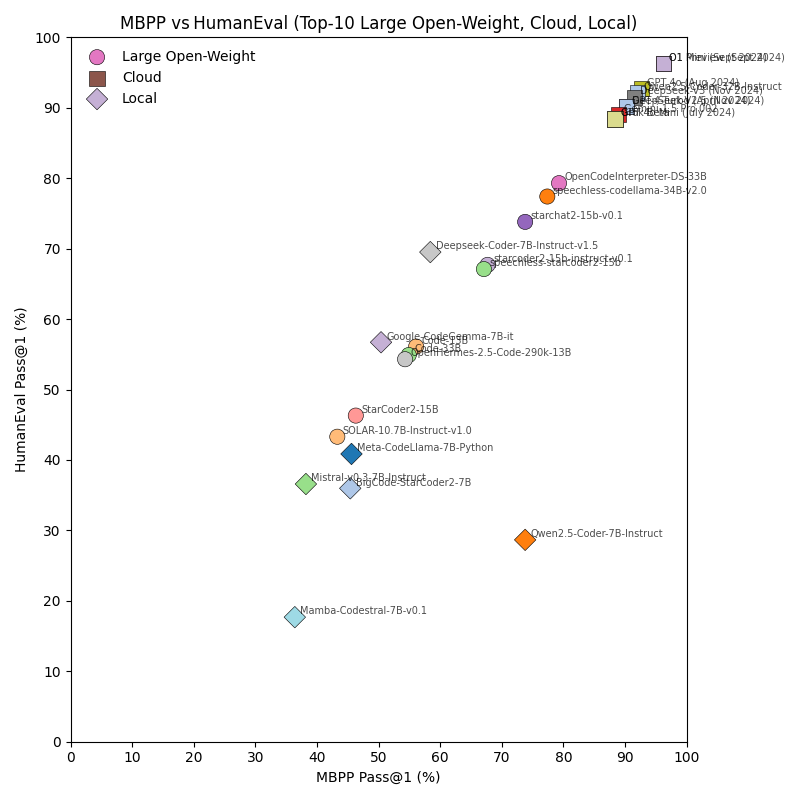
\includegraphics[width=\linewidth]{graphics/scatter_mbpp_vs_humaneval.png}
			\captionof{figure}{MBPP vs HumanEval Pass@1 scores}
			\label{fig:scatter-scores}
		\end{minipage}
		\hfill
		\begin{minipage}[t]{0.48\linewidth}
			\centering
			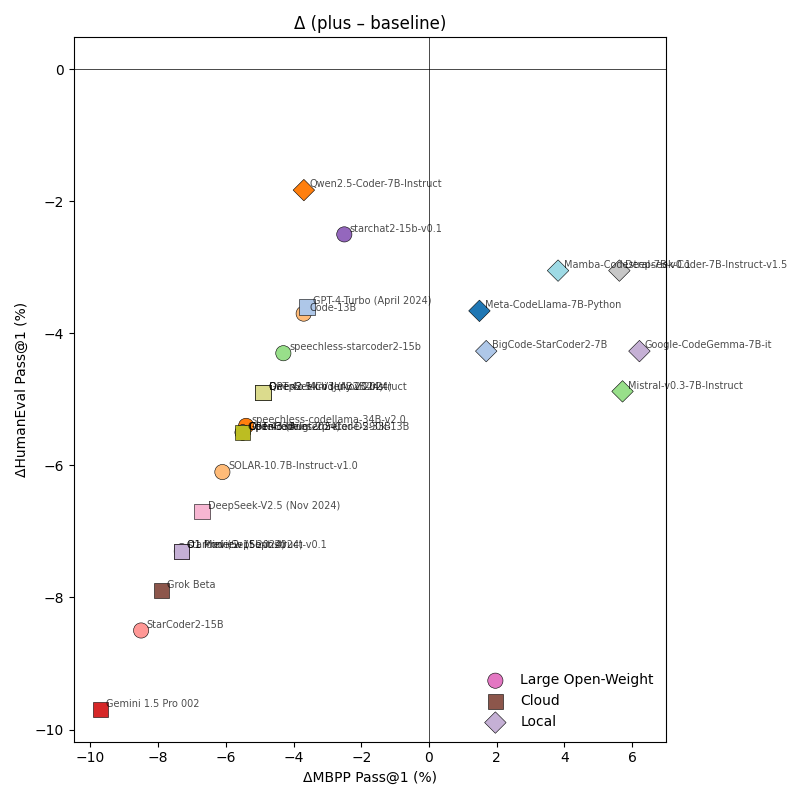
\includegraphics[width=\linewidth]{graphics/scatter_deltas_mbpp_vs_humaneval.png}
			\captionof{figure}{Base vs augmented Pass@1 score deltas}
			\label{fig:scatter-deltas}
		\end{minipage}
	\end{center}

	\section{Conclusions}
	The evaluation confirms that modern self-hosted LLMs can serve as viable, secure alternatives to proprietary cloud-based AI models for code generation. Their performance, privacy benefits, and deployment feasibility collectively support an affirmative answer to the central research question.

	\textbf{Key Findings:}
	\begin{enumerate}[label=SQ\arabic*., ref=SQ\arabic*]
		\item Qwen2.5 achieved top MBPP scores, while Deepseek delivered more consistent results across all benchmarks.
		\item Both models produced reliable, secure code, though oversight remains necessary to catch edge-case vulnerabilities.
		\item Performance approached that of leading cloud models, though a noticeable gap remains in complex tasks.
		\item Local deployment required capable GPUs and technical expertise, but proved sustainable and reproducible.
		\item Effective use requires reproducible setups and preserving human oversight and auditability throughout deployment.
	\end{enumerate}

	Self-hosted LLMs have matured into practical tools for privacy-conscious enterprises, offering robust performance without relying on external providers.

	\section{Future Research}
	Future work should explore LoRA-based fine-tuning for task-specific adaptation, hybrid local–cloud deployment strategies, and safety-focused evaluation protocols. Self-hosted models have evolved from a theoretical concept into a practical, deployable alternative to cloud-based solutions.

\end{multicols}
\end{document}